\documentclass[12pt]{article}

\usepackage{amssymb,amsmath,amsthm}
\usepackage{graphicx} % Package for including figures
%\usepackage{psfrag,color}

\title{Automation and Scripting: Lab 1 Math/CS 471}
\author{AUTHOR1 and AUTHOR2}
\date{today}   % Activate to display a given date or no date


\begin{document}
\maketitle

\begin{abstract}
Brief summary of your report.
\end{abstract}
\section{Introduction}
\LaTeX is a useful tool to typset reports, papers and other
scientific documents. 

\subsection{Equations}
It has very powerful support for equations such
as these:
\begin{equation}
f(x) = e^{1/2 - \sin(5 \pi    x)}, \label{eq:1} 
\end{equation}
\begin{equation}
p(x) = 1+x+x^2. \label{eq:2} 
\end{equation}

\subsection{Referencing}
\LaTeX also supports a very convenient labeling / referencing system
through the commands \verb+\label / \ref+ . Above, equation
(\ref{eq:2}) is a polynomial and the function described by equation
(\ref{eq:1}) is plotted in Figure \ref{fig:1}. 

{\bf Note} that you may have to compile the document two times to get
all the cross-referencing to work correctly.

\subsection{Figures}
Figures are also easy to incorporate. It is often best to use a figure
format that is based on vector graphics, e.g. Encapsulated PostScript
(eps). An example is given in Figure \ref{fig:1} where equation
(\ref{eq:1}) is displayed.

\begin{figure}[htb]
\begin{center}
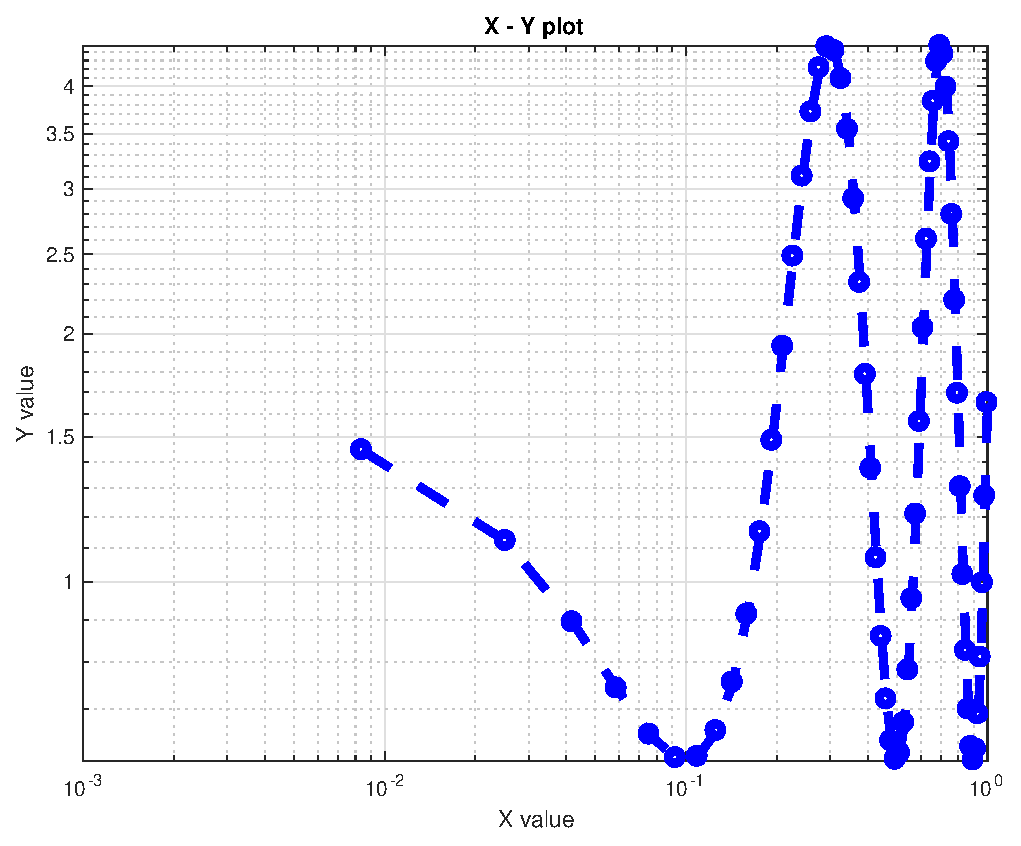
\includegraphics[width=0.32\textwidth]{lab1.eps}
\caption{This figure displays the function $f(x) = e^{1/2 - \sin(5 \pi
    x)}$. \label{fig:1}}
\end{center}
\end{figure}

\subsection{Tables}
Tables are often useful to display data more compactly than figures.

\begin{table}[h]
\begin{centering}
  \begin{tabular}{| l | c |}
   \hline 
   Breakfast & Spam \\
Lunch & Sausage \\
Dinner & Potatoes \\
  
   \hline
  \end{tabular}
  \caption{A table of delicious meals. \label{tab:1}}
  \end{centering}
\end{table}

\subsection{Tables 2}
This is the modified new table 

\begin{table}[h]
\begin{centering}
  \begin{tabular}{| l | c |}
   \hline 
   Breakfast & Very important \\
Lunch & Important \\
Dinner & Less important \\
  
   \hline
  \end{tabular}
  \caption{The importance of each meal. \label{tab:2}}
  \end{centering}
\end{table}
%\bibliographystyle{plain}
%\bibliography{bibfile}

\end{document}  
